%! Author = ben
%! Date = 16/02/2021


%%%%%%%%%%%%%% 16/02/2020 %%%%%%%%%%%%%%%%
\subsection*{\textbf{16/02/2020}}
%%%%%%%%%%%%% 9:00 %%%%%%%%%%%%%
\subsubsection*{\textbf{09:00}}
Discussion of plan for the day:
\begin{itemize}
    \item Finish plotting $Z \rightarrow ll$ plots
    \item Apply cuts to pTCone30 plots
    \item etCone20 plots
\end{itemize}

%%%%%%%%%%%%% 09:23 %%%%%%%%%%%%%
\subsubsection*{09:23 - Lead DG}
Plot etcone20 to investigate what data is available.
\\
Figure.\ref{fig:Zee-fast_ETcone20(0)_0-15GeV_16-02-21_09-34}


plots Fig.\ref{fig:Zee-fast_ETcone20(1)_0-15GeV_16-02-21_09-41} of the etcone20(1)

\\
Both fig.\ref{fig:Zee-fast_ETcone20(0)_0-15GeV_16-02-21_09-34} and fig.\ref{fig:Zee-fast_ETcone20(1)_0-15GeV_16-02-21_09-41} are similar with a larger mean value for fig.\ref{fig:Zee-fast_ETcone20(1)_0-15GeV_16-02-21_09-41}.
\\
Noticed a "bump" at around 4 GeV.
\\
Plan to plot the log of the data to investigate if decay is related to exponential decay.
\begin{figure}[h!]
    \centering
    \begin{minipage}{0.5\textwidth}
        \centering
        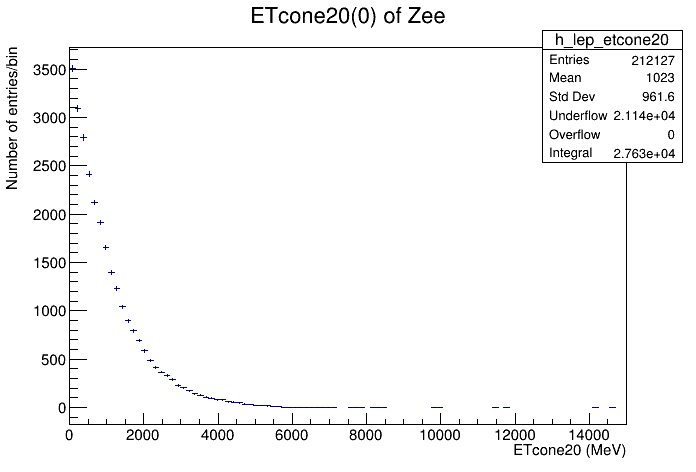
\includegraphics[width=\linewidth]{plots/16-02-2021/Zee-fast_ETcone20(0)_0-15GeV_16-02-21_09-34}
        (A)
    \end{minipage}\hfill
    \begin{minipage}{0.5\textwidth}
        \centering
        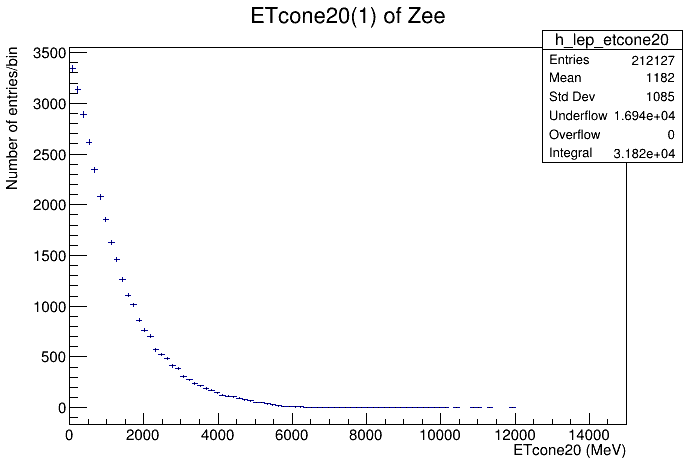
\includegraphics[width=\linewidth]{plots/16-02-2021/Zee-fast_ETcone20(1)_0-15GeV_16-02-21_09-41}
        (B)
    \end{minipage}
    \caption{ (A) Plot of $Z \rightarrow ee$ ETCone20(0) for Zee-fast MC data. (B) Plot of  $Z \rightarrow ee$ ETCone20(1) for Zee-fast MC data.}
    \label{fig:}
\end{figure}

%%%%%%%%%%%%% 09:53 %%%%%%%%%%%%%
\subsubsection*{09:53}
Plotting the ETCone of each of the two leptons produced from the decay of $Z \rightarrow \mu \mu$ using the MC data.
\begin{figure}[h!]
    \centering
    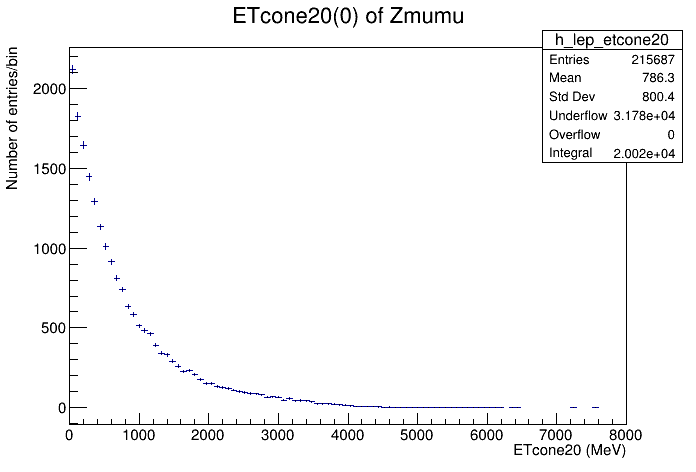
\includegraphics[width=0.85\linewidth]{plots/16-02-2021/Zmumu-fast_ETcone(0)_0-8GeV_16-02-21_09-54.png}
    \caption{Plot of  $Z \rightarrow \mu\mu$ ETCone20(0) for $Z\mu\mu$-fast MC.  data.}\label{fig:Zmumu-fast_ETcone(0)_0-8GeV_16-02-21_09-54}
\end{figure}
On fig\ref{fig:Zmumu-fast_ETcone(0)_0-8GeV_16-02-21_09-54} a slight "bump" at around 1.9 GeV

\begin{figure}[h!]
    \centering
    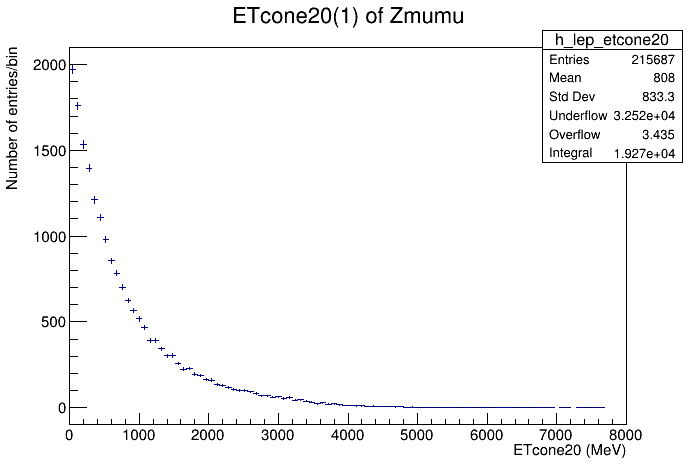
\includegraphics[width=0.85\linewidth]{plots/16-02-2021/Zmumu-fast_ETcone(1)_0-8GeV_16-02-21_09-56.png}
    \caption{Plot of  $Z \rightarrow \mu\mu$ ETCone20(1) for $Z\mu\mu$-fast MC.  data.}\label{fig:Zmumu-fast_ETcone(1)_0-8GeV_16-02-21_09-56}
\end{figure}
On fig.\ref{fig:Zmumu-fast_ETcone(1)_0-8GeV_16-02-21_09-56} the

%%%%%%%%%%%%% 10:07 %%%%%%%%%%%%%
\subsubsection*{10:07}
Plotting the pTCone30 (0)\&(1) of $Z\rightarrow ee$ for the range of 1-4 GeV. This range is used due to 0-1 GeV not being detected. (See 11-02-2021 for the investigation and plots of the full energy range.)

\begin{figure}[h!]
    \centering
    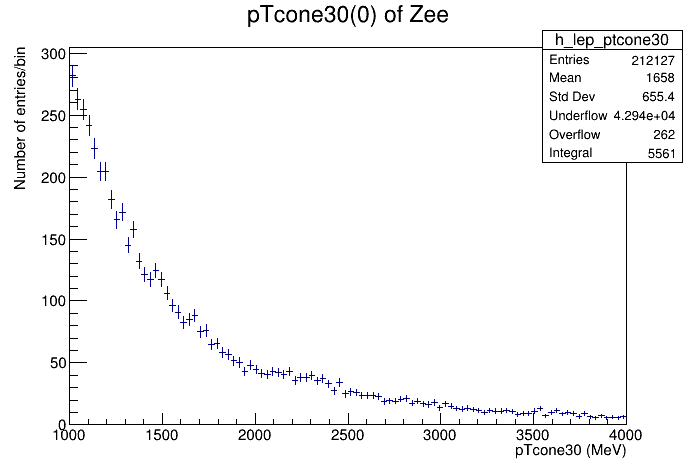
\includegraphics[width=0.85\linewidth]{plots/16-02-2021/Zee_fast_pTcone30(0)_1-4GeV_16-02-21_10-07.png}
    \caption{Plot of  $Z \rightarrow \mu\mu$ pTcone30(0) for $Z\rightarrow ee$-fast MC.  data.}\label{fig:/Zee_fast_pTcone30(0)_1-4GeV_16-02-21_10-07}
\end{figure}

On fig.\ref{fig:/Zee_fast_pTcone30(0)_1-4GeV_16-02-21_10-07}, the number of entries decrease exponentially as momentum increases.  There is also a "bump" around pTcone30 = 2.25GeV

\begin{figure}[h!]
    \centering
    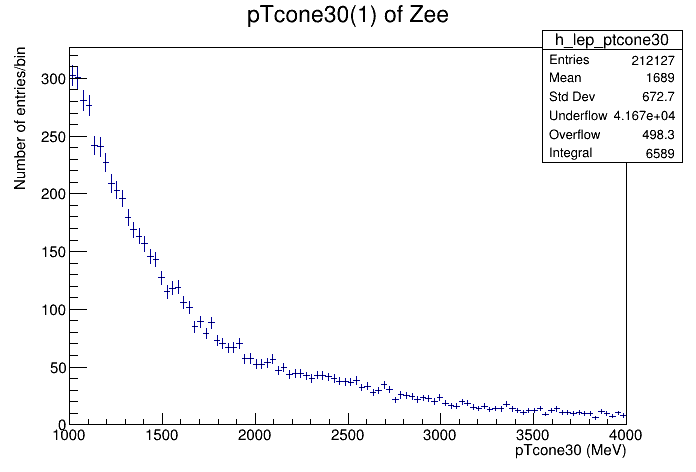
\includegraphics[width=0.85\linewidth]{plots/16-02-2021/Zee_fast_pTcone30(1)_1-4GeV_16-02-21_10-12.png}
    \caption{Plot of  $Z \rightarrow \mu\mu$ pTcone30(1) for $Z\rightarrow ee$-fast MC.  data.}\label{fig:Zee_fast_pTcone30(1)_1-4GeV_16-02-21_10-12}
\end{figure}

In fig.\ref{fig:Zee_fast_pTcone30(1)_1-4GeV_16-02-21_10-12} to "bump" seen is not as pronounced as in fig.\ref{fig:/Zee_fast_pTcone30(0)_1-4GeV_16-02-21_10-07}.


%%%%%%%%%%%%% 10:18 %%%%%%%%%%%%%
\subsubsection*{10:18}
Plotting the pTCone30 (0)\&(1) of $Z\rightarrow \mu\mu$ for the range of 1-4 GeV. This range is used due to 0-1 GeV not being detected. (See 11-02-2021 for the investigation and plots of the full energy range.)

\begin{figure}[h!]
    \centering
    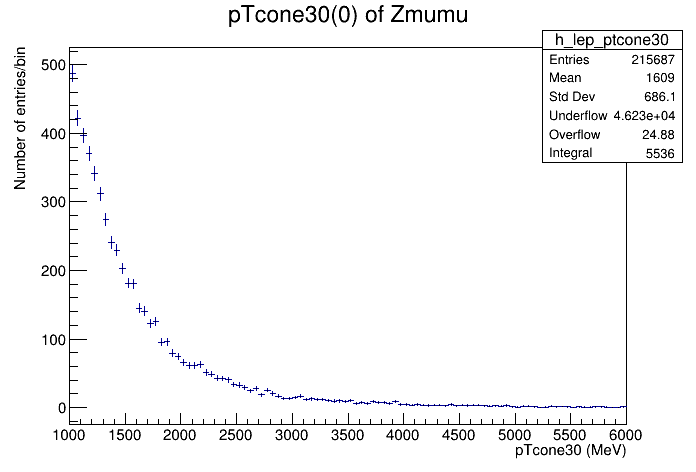
\includegraphics[width=0.85\linewidth]{plots/16-02-2021/Zmumu_fast_pTcone30(0)_1-6GeV_16-02-21_10-18.png}
    \caption{Plot of  $Z \rightarrow \mu\mu$ pTcone30(0) for $Z\mu\mu$-fast MC.  data.}\label{fig:Zmumu_fast_pTcone30(0)_1-6GeV_16-02-21_10-18}
\end{figure}

\begin{figure}[h!]
    \centering
    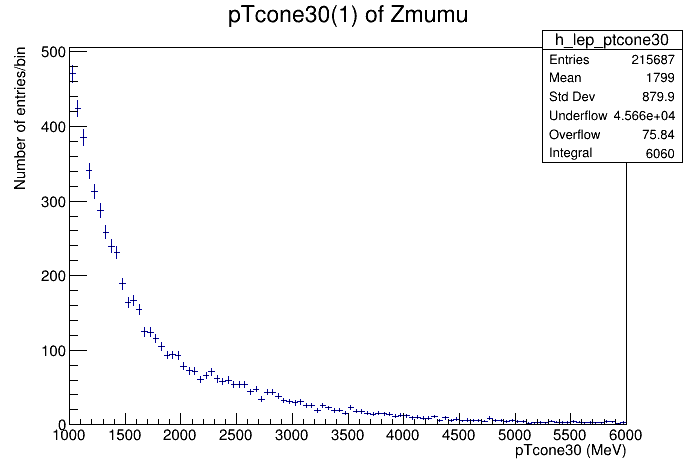
\includegraphics[width=0.85\linewidth]{plots/16-02-2021/Zmumu_fast_pTcone30(1)_1-6GeV_16-02-21_10-21.png}
    \caption{Plot of  $Z \rightarrow \mu\mu$ pTcone30(1) for $Z\mu\mu$-fast MC.  data.}\label{fig:Zmumu_fast_pTcone30(1)_1-6GeV_16-02-21_10-21}
\end{figure}


%%%%%%%%%%%%% 10:40 %%%%%%%%%%%%%
\subsubsection*{10:40}
Plotting the pTcone30 (total (sum of the two leptons)) of ATLAS data with cuts:
\begin{itemize}
    \item opposite charge
    \item lep\_type == 11 (lepton type = electron)
    \item lep\_n == 2 (number of leptons = 2)
\end{itemize}
To start, plot the range of 0-10 GeV to show 0-1 GeV is not detected.  This is seen in Fig.\ref{fig:2lep_fast_ee-pair_pTcone30(total)_0-10GeV_16-02-21_10-50} with a peak value at (total) pTcone30
\begin{figure}[h!]
    \centering
    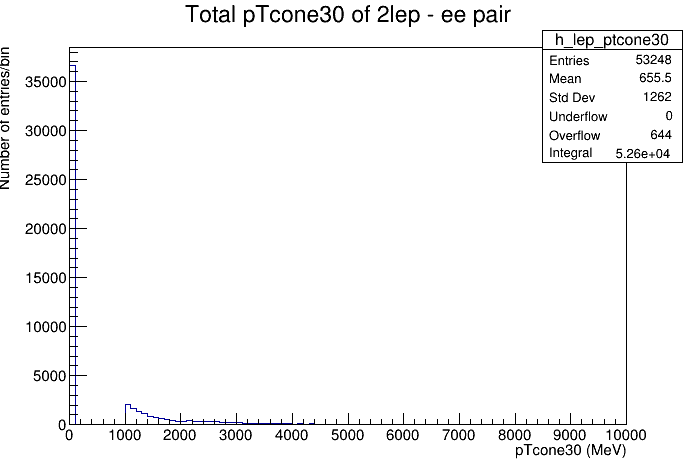
\includegraphics[width=0.85\linewidth]{plots/16-02-2021/2lep_fast_ee-pair_pTcone30(total)_0-10GeV_16-02-21_10-50}
    \caption{Plot of  $Z \rightarrow \mu\mu$ pTcone30(1) for $Z\mu\mu$-fast MC.  data.}\label{fig:2lep_fast_ee-pair_pTcone30(total)_0-10GeV_16-02-21_10-50}
\end{figure}


\begin{figure}[h!]
    \centering
    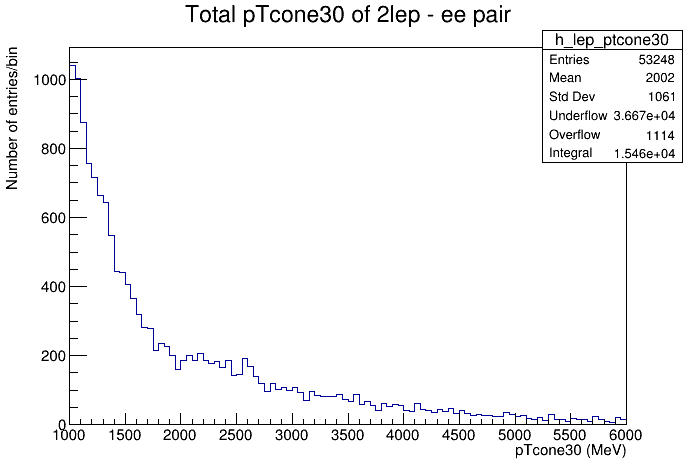
\includegraphics[width=0.85\linewidth]{plots/16-02-2021/2lep_fast_ee-pair_pTcone30(total)_1-6GeV_16-02-21_10-59}
    \caption{Plot of  $Z \rightarrow \mu\mu$ pTcone30(1) for $Z\mu\mu$-fast MC.  data.}\label{fig:2lep_fast_ee-pair_pTcone30(total)_1-6GeV_16-02-21_10-59}
\end{figure}

Fig.\ref{fig:2lep_fast_ee-pair_pTcone30(total)_1-6GeV_16-02-21_10-59} has the range set to 1-6 GeV (to remove the un-detected regoin 0-1 GeV).  This still shows exponential like decay as pTcone increases. \\
The "bump"/inconsistency (if expecting smooth exponential like decay) is present in the experiental ATLAS data around 2-2.7 GeV.  To investigate this bump, plan to plot the invariant mass with a cut to select for a pTcone30 in the vicinity of 2-2.7 GeV.

%%%%%%%%%%%%% 11:10 %%%%%%%%%%%%%
\subsubsection*{11:10}
Plotting ATLAS 2lep data for the total ETCone20 for a ee pair in the range of 0-6 GeV.  This can be seen in Fig.\ref{fig:2lep_fast_ee-pair_ETcone30(total)_0-6GeV_16-02-21_11-11}

\begin{figure}[h!]
    \centering
    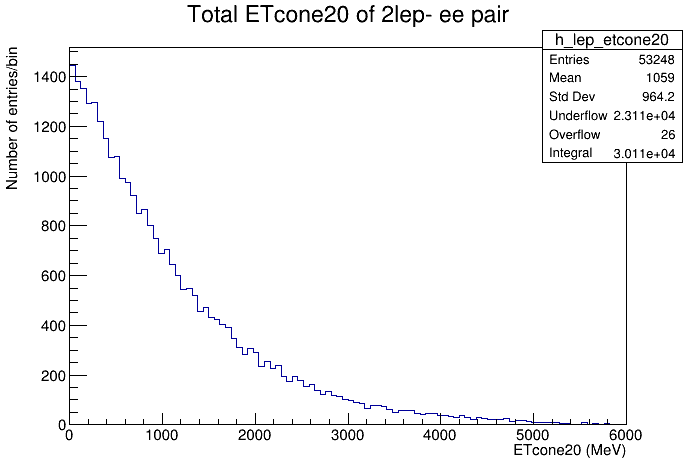
\includegraphics[width=0.85\linewidth]{plots/16-02-2021/2lep_fast_ee-pair_ETcone30(total)_0-6GeV_16-02-21_11-11}
    \caption{Plot of the total ETCone20 of an ee pair using the 2lep-fast ATLAS data.  data.}\label{fig:2lep_fast_ee-pair_ETcone30(total)_0-6GeV_16-02-21_11-11}
\end{figure}

%%%%%%%%%%%%% 11:14 %%%%%%%%%%%%%
\subsubsection*{11:14}

\begin{figure}[h!]
    \centering
    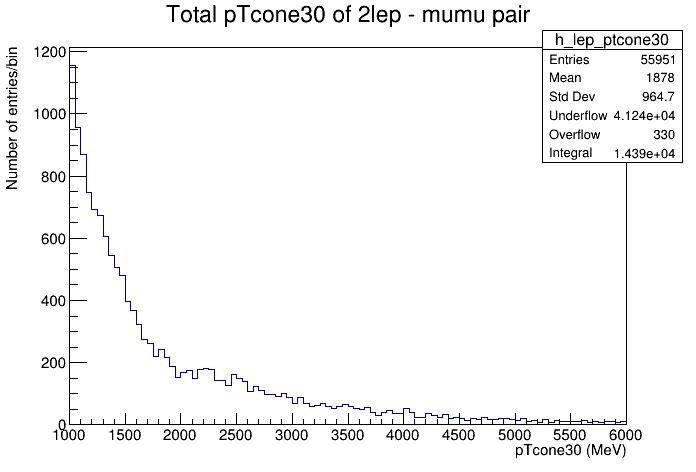
\includegraphics[width=0.85\linewidth]{plots/16-02-2021/2lep_fast_mumu-pair_pTcone30(total)_1-6GeV_16-02-21_11-06}
    \caption{Plot of the total pTcone30 of a mumu pair using the 2lep-fast ATLAS data. }\label{fig:2lep_fast_mumu-pair_pTcone30(total)_1-6GeV_16-02-21_11-06}
\end{figure}

\begin{figure}[h!]
    \centering
    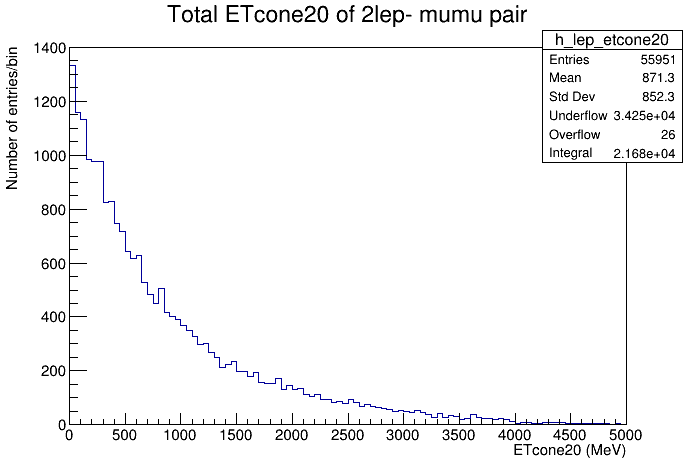
\includegraphics[width=0.85\linewidth]{plots/16-02-2021/2lep_fast_mumu-pair_ETcone30(total)_0-5GeV_16-02-21_11-14}
    \caption{Plot of the total ETcone20 of a mumu pair using the 2lep-fast ATLAS data. }\label{fig:2lep_fast_mumu-pair_ETcone30(total)_0-5GeV_16-02-21_11-14}
\end{figure}



%%%%%%%%%%%%% 11:24 %%%%%%%%%%%%%
\subsubsection*{11:24 - Lead BG}
To investigate the possible bump or dip (as seen in the pTcone30 data (bump around \dots  or dip around \dots)) plot the log of the ptCone30.


%2lep mumu logs


%pTcone
\begin{figure}[h!]
    \centering
    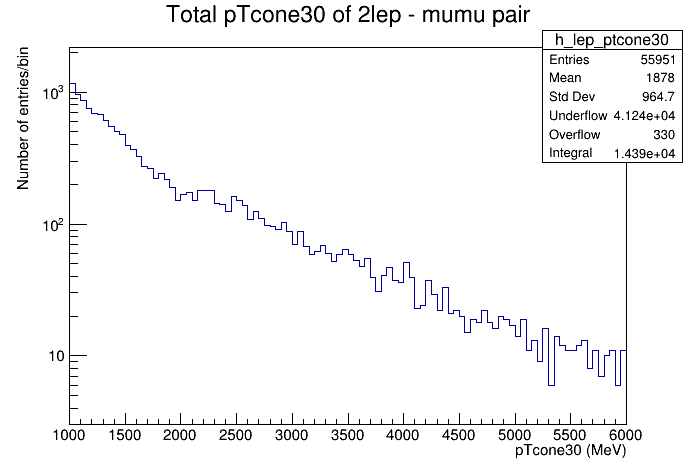
\includegraphics[width=0.85\linewidth]{plots/16-02-2021/2lep-fast_mumu_ptcone30(total)_log-entries_1-6GeV_16-02-2021_11-39}
    \caption{Plot of the total pTcone30 of a mumu pair using the 2lep-fast ATLAS data, log. }\label{fig:2lep-fast_mumu_ptcone30(total)_log-entries_1-6GeV_16-02-2021_11-39}
\end{figure}




\begin{figure}[h!]
    \centering
    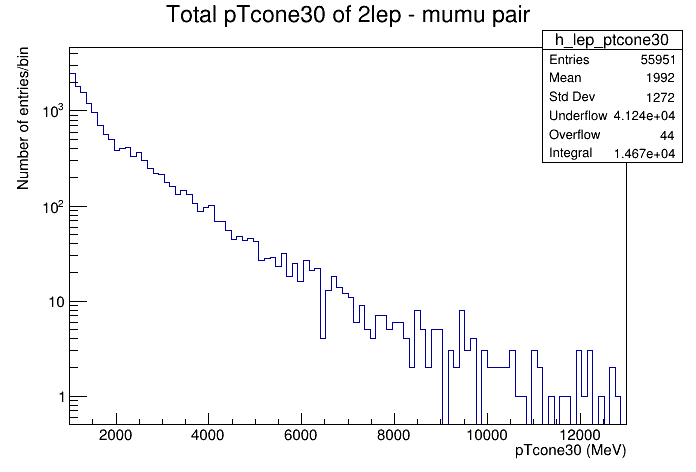
\includegraphics[width=0.85\linewidth]{plots/16-02-2021/2lep-fast_mumu-pair_ptcone30(total)_log-entries_1-13GeV_16-02-2021_11-45}
    \caption{Plot of the total pTcone30 of a mumu pair using the 2lep-fast ATLAS data, log,1-13GeV. }\label{fig:2lep-fast_mumu-pair_ptcone30(total)_log-entries_1-13GeV_16-02-2021_11-45}
\end{figure}

\begin{figure}[h!]
    \centering
    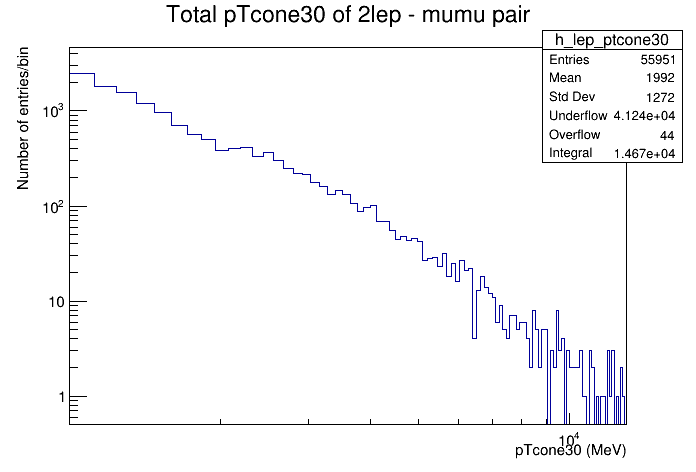
\includegraphics[width=0.85\linewidth]{plots/16-02-2021/2lep-fast_mumu-pair_ptcone30(total)_log-log_1-13GeV_16-02-2021_11-45}
    \caption{Plot of the total pTcone30 of a mumu pair using the 2lep-fast ATLAS data, log-log,1-13GeV. }\label{fig:2lep-fast_mumu-pair_ptcone30(total)_log-log_1-13GeV_16-02-2021_11-45.png}
\end{figure}


%ETcone
\begin{figure}[h!]
    \centering
    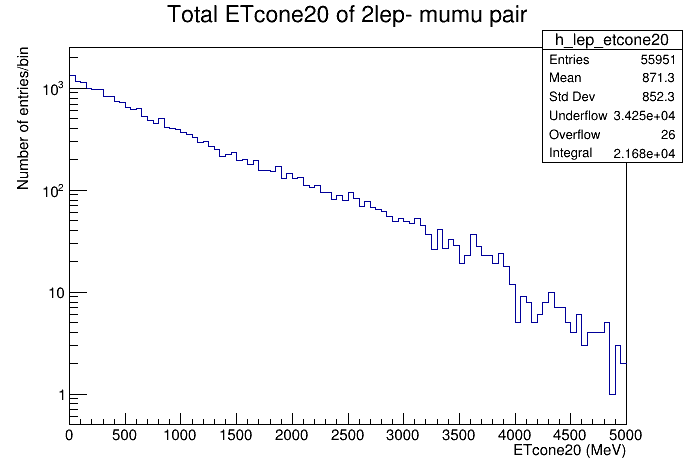
\includegraphics[width=0.85\linewidth]{plots/16-02-2021/2lep-fast_mumu-pair_etcone20(total)_log-entries_0-5GeV_16-02-2021_11-31}
    \caption{Plot of the total ETcone20 of a mumu pair using the 2lep-fast ATLAS data, log, 0-5GeV. }\label{fig:2lep-fast_mumu-pair_etcone20(total)_log-entries_0-5GeV_16-02-2021_11-31}
\end{figure}

\begin{figure}[h!]
    \centering
    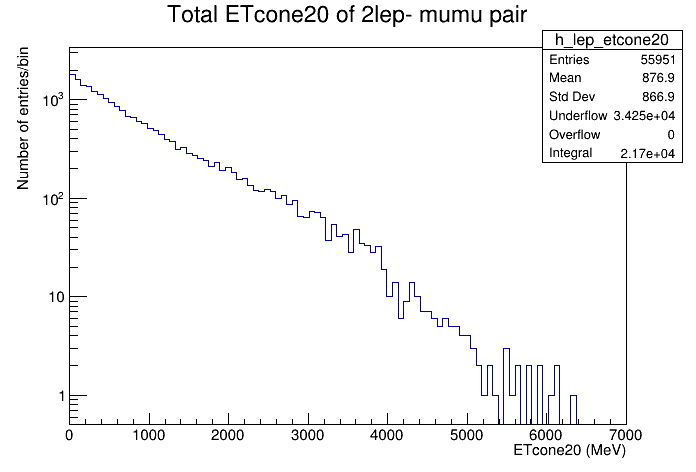
\includegraphics[width=0.85\linewidth]{plots/16-02-2021/2lep-fast_mumu-pair_etcone20(total)_log-entries_0-7GeV_16-02-2021_11-33.png}
    \caption{Plot of the total ETcone20 of a mumu pair using the 2lep-fast ATLAS data, log,0-7GeV. }\label{fig:2lep-fast_mumu-pair_etcone20(total)_log-entries_0-7GeV_16-02-2021_11-33}
\end{figure}

\subsection*{14:06- BG lead}\\
Investigate use of stacked MC plots to identify background when comparing to ATLAS data.//

\subsection*{14:50}\\
Stacked plot made for invariant. mass

\subsubsection*{16:20}
Stacked plot made for mean etcone20, includes
\begin{itemize}
    \item 2lep data
    \item Zee MC
    \item Zmumu MC
    \item Ztautau MC
\end{itemize}

\begin{figure}[h!]
    \centering
    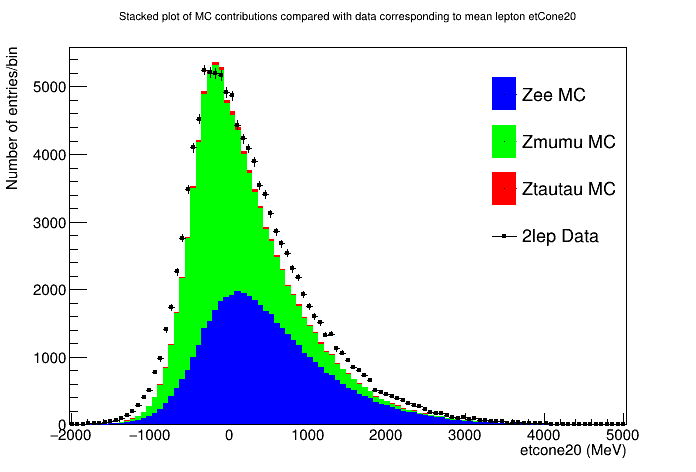
\includegraphics[width=0.85\linewidth]{plots/16-02-2021/2lep-Zee-Zmumu-Ztautau-fast_mean-etcone20_-2-5GeV_16-02-21_16-28}
    \caption{Stack plot of the mean ETcone20 of 2 lep with opposite charge pair using the 2lep-fast ATLAS data, log,0-7GeV. }\label{fig:2lep-Zee-Zmumu-Ztautau-fast_mean-etcone20_-2-5GeV_16-02-21_16-28}
\end{figure}


\subsubsection*{16:28}
Unexplained discrepancy of 2lep data around peak ~$0$MeV (Fig.\ref{fig:2lep-Zee-Zmumu-Ztautau-fast_mean-etcone20_-2-5GeV_16-02-21_16-28})